\section{A fixed atom index is part of the physics}\label{sec:identity}
A rare-event method compares two geometries atom by atom.
The path, the tangent, the displacement, the Hessian and the rate are defined only when atom \(i\) in image A is atom \(i\) in image B.
Write the \(3N\) Cartesian coordinates of an image, in one fixed order, as the vector \(R\).
The improved NEB tangent at image \(i\) is built from the forward and backward differences
\begin{equation}
\label{eq:tangent}
\tau_i^{+}=R_{i+1}-R_i,\qquad \tau_i^{-}=R_i-R_{i-1},
\end{equation}
and the spring force lies along that tangent
\cite{jonssonNudgedElasticBand1998,henkelmanImprovedTangentEstimate2000},
\begin{equation}
\label{eq:spring}
F_i^{\parallel}=k\big(|R_{i+1}-R_i|-|R_i-R_{i-1}|\big)\,\hat\tau_i.
\end{equation}
A permutation matrix \(\Pi\) applied to one image replaces \(R\) by \(\Pi R\).
The differences in Eq.~\eqref{eq:tangent} then connect different atoms, and the spring in Eq.~\eqref{eq:spring} pulls along that wrong chord.
The Cartesian RMSD between reactant and product has the same dependence,
\begin{equation}
\label{eq:rmsd}
\mathrm{RMSD}^{2}(R^{\mathrm{R}},R^{\mathrm{P}})=\frac{1}{N}\sum_{a=1}^{N}\big|r_a^{\mathrm{R}}-r_a^{\mathrm{P}}\big|^{2}.
\end{equation}
The sum is a distance between matched atoms.
The permutation-invariant distance minimises Eq.~\eqref{eq:rmsd} over rotations and over the \(M_1!M_2!\cdots\) maps of identical elements
\cite{sadeghiMetricsConfigurationSpace2013,deFindingReactionPathways2019,goswamiTwodimensionalRmsdProjections2026}.
Two-sided searches need that map before the first image is placed
\cite{deFindingReactionPathways2019,goswamiReproducibleOrchestrationBest2026}.
The image-dependent pair potential builds its target from the distances \(d_{ab}\) of a chosen map and then runs NEB on that objective
\cite{smidstrupImprovedInitialGuess2014}.
A wrong map asks the band to turn the wrong pairs of atoms into neighbours.
Harmonic transition-state theory has the same index.
The Vineyard prefactor, Eq.~\eqref{eq:vineyard}, is a ratio of frequencies of the free Cartesian modes.
Those modes are eigenvectors of the mass-weighted Hessian in the order of \(R\).
A permutation reorders the Hessian, and a mask that frees one more component changes which eigenvalues enter the products.

A file that stores coordinates and element symbols, and no atom index, leaves the map to the next program.
An XYZ written and read through a SMILES canonicalisation, an Open Babel conversion or an RDKit molecule rebuild can return the atoms in a new order.
A POSCAR groups atoms by the element block.
A LAMMPS dump written with atoms sorted by type does the same.
In each case Eq.~\eqref{eq:tangent} is evaluated on a vector whose slots no longer name the atoms of the previous image.
The band still returns a number.
That number is the barrier of a different path.

\section{The Claisen rearrangement}\label{sec:claisen}
Allyl vinyl ether rearranges to pent-4-enal by a [3,3] sigmatropic shift
\cite{bakerLocationTransitionStates1996}.
The reactant and the product are the same fourteen atoms.
The path breaks one C--O bond and forms one C--C bond through a six-membered chair.
The endpoints are the benchmark CON frames, used as written.
Energies and forces are PET-MAD-S, version 1.1.0, through metatomic
\cite{mazitovPETMADLightweight2025,bigiMetatensorMetatomicFoundational2026}.
The band is an OCI-NEB with a climbing image
\cite{henkelmanClimbingImageNudged2000}, run in eOn 3.6.0 on one CPU
\cite{rohitgoswamiTheochemuieonV3602026}.

Label the atoms once, in the reactant.
The product coordinates \(R^{\mathrm{P}}\) in that same label enter the linear image
\begin{equation}
\label{eq:lerp}
R(s)=(1-s)\,R^{\mathrm{R}}+s\,R^{\mathrm{P}},\qquad s\in[0,1].
\end{equation}
The path length of Eq.~\eqref{eq:lerp} is \(|R^{\mathrm{P}}-R^{\mathrm{R}}|\).
A second labelling \(\Pi\) of the product replaces the length by \(|\Pi R^{\mathrm{P}}-R^{\mathrm{R}}|\).
The NEB tangent and the spring, Eqs.~\eqref{eq:tangent} and~\eqref{eq:spring}, then follow whatever nuclei the new slots happen to pair.

The chemical correspondence is the identity permutation carried by the atom ids of the two frames.
That band converges.
It has ten images and takes 453 force calls, and the climbing-image force is \(0.042\,\mathrm{eV/\text{\AA}}\).
The barrier is 0.607~eV (14.0~kcal/mol).
The highest image is a connected six-membered chair (Figure~\ref{fig:claisen-struct}).
The forming distance C5--C0 is \(2.046\,\text{\AA}\) and the breaking distance C2--O is \(1.488\,\text{\AA}\).
One internal mode is imaginary, at \(-542.5\,\mathrm{cm}^{-1}\).

IRA reassigns the same product by the rotation and the permutation that minimise the Hausdorff distance, with \(k_{\max}\) factor 3
\cite{gundeIRAShapeMatching2021}.
The permutation is \([0,4,3,1,2,5,6,7,11,12,13,9,8,10]\), and it moves 10 of the 14 atoms.
The Hausdorff distance is \(2.109\,\text{\AA}\).
Equation~\eqref{eq:rmsd} after the Kabsch rotation is \(1.443\,\text{\AA}\) on this map and \(1.519\,\text{\AA}\) on the identity map.
The shorter distance pairs the wrong nuclei for the [3,3] shift.

The band on that product has eighteen images (Figure~\ref{fig:claisen-band}).
Its force remains above \(0.05\,\mathrm{eV/\text{\AA}}\).
The lowest value is \(0.189\,\mathrm{eV/\text{\AA}}\), at iteration 362.
The highest image lies at 3.988~eV (92.0~kcal/mol).
The atoms have separated into C0--C1--C2\({=}\)O and a detached C4--C5, with O--C4 at \(2.874\,\text{\AA}\) (Figure~\ref{fig:claisen-struct}).
Three internal modes are imaginary, at \(-251\), \(-135\) and \(-123\,\mathrm{cm}^{-1}\).
The image is a higher-order stationary point.
The images of Eq.~\eqref{eq:lerp} on this permutation drag atoms through one another, because a slot in \(R^{\mathrm{P}}\) holds a different nucleus from the slot in \(R^{\mathrm{R}}\).

A swap of H11 with H13, and no other change of label, produces a band different from the [3,3] map.
The minimum-Hausdorff assignment minimises a distance.
The chemical map is the atom id, and that id has to travel with the coordinates.
A CON row stores the id beside the position, and readcon returns the id with the position.

\begin{figure}[tbp]
\centering
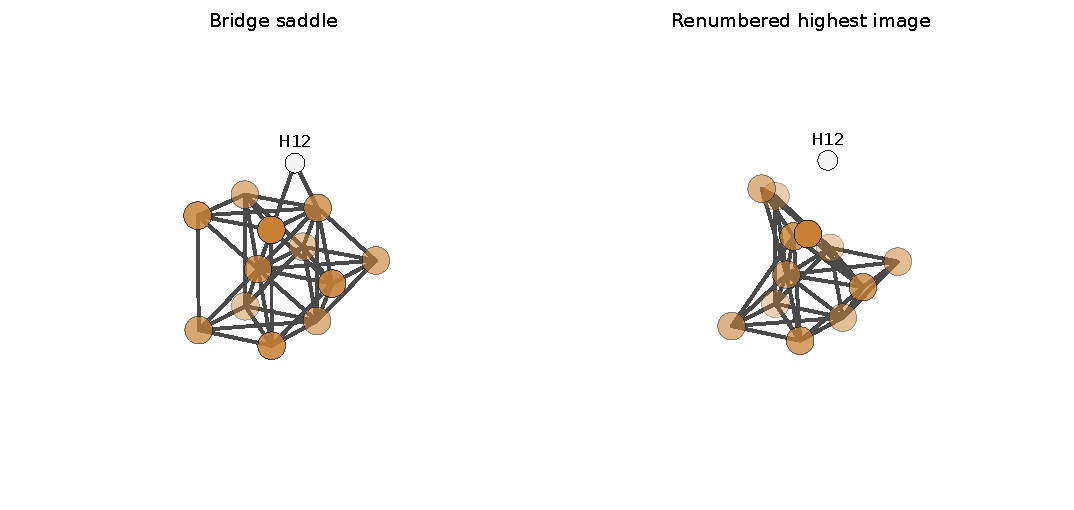
\includegraphics[width=\textwidth]{figures/generated/claisen_structures.pdf}
\caption{Highest image of each band, drawn from the CON coordinates.
(a)~The connected six-membered chair of the chemical map.
The dashed segment is the forming C5--C0 contact.
(b)~The highest image of the Hausdorff reassignment, with C0--C1--C2\({=}\)O separated from C4--C5.
Labels are the atom ids stored on the rows.
Carbon is grey, oxygen red and hydrogen white.}
\label{fig:claisen-struct}
\end{figure}

\begin{figure}[tbp]
\centering
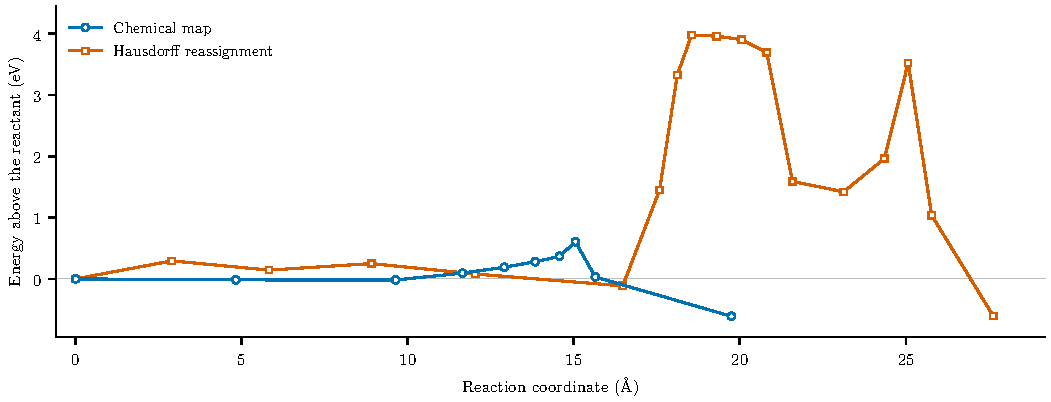
\includegraphics[width=\textwidth]{figures/generated/claisen_band.pdf}
\caption{Final bands for allyl vinyl ether to pent-4-enal.
Energy of each image above the reactant, on one reaction coordinate.
Circles follow the chemical correspondence carried by the atom ids.
Squares follow the minimum-Hausdorff reassignment of the product.}
\label{fig:claisen-band}
\end{figure}

\section{The same atom in the next frame}\label{sec:connectivity}
The published d-SEAMS analyses read LAMMPS dump text.
seams-core also reads a \texttt{.con} file through readcon-core.
\texttt{sinp::readCon} takes one frame, and \texttt{cloudFromHandle} copies each atom into the point cloud.
\texttt{Point::type} is the atomic number from the file.
\texttt{Point::atomID} is the file's \texttt{atom\_id}.
\texttt{mapAtomIdToIndex} records that id against the cloud index, so a later lookup uses the id and not the row the file happened to write.
A sheared CON cell, lengths and angles, is stored as the same triclinic box a LAMMPS tilt dump carries: the three lengths and the \(xy\), \(xz\) and \(yz\) tilts.

XYZ, as d-SEAMS reads it, has no atom id, so the id is the file order.
Every XYZ atom is stored as type 1, and the comment line is not read as a cell.
A LAMMPS dump carries an id column and a box only when the dump was written with them.
A \texttt{.con} frame carries the id, the element and the triclinic cell on every frame.
A per-atom result then joins the next frame, and a frame in a corpus, by that id.

d-SEAMS uses that id for quasi-one-dimensional nanotube water.
\texttt{ring::rmAxialTranslations} finds the same atom in a later frame through the id-to-index map and shifts the tube along its axis.
The per-atom record is one line of frame, atom id, \(c_{ij}\) and ice type.

readcon-db ingests a \texttt{.con} trajectory into an LMDB corpus.
seams-core selects that corpus by element or by formula, across the shard roots of a campaign, and decodes the \(N\)th hit with the same reader.

\noindent\textbf{Placeholder for the mW water demo.}
The demo reads ring and hydrogen-bond persistence by id from a \texttt{.con} trajectory, the same trajectory written as XYZ and shuffled in frame order, and the round trip through readcon-db.
The figure and the numbers are not in this draft.
No value is stated here.

\section{The fields the rate actually reads}\label{sec:fields}
CON 3.1 stores, on each frame, the coordinates, the cell, the periodic flags, a three-bit mask, an integer identifier, the mass, and, from minor 1, the velocities with a declared time unit.
Each field is an input of one of the equations above.

The identifier is the index \(a\) in Eq.~\eqref{eq:rmsd} and the slot of \(R\) in Eq.~\eqref{eq:tangent}.
It is written on the coordinate row, so a later file that groups rows by element still names the same atom.
The mask deletes Cartesian components from the free set \(n\) in Eq.~\eqref{eq:vineyard}.
A constrained dimer or a constrained band holds those components fixed.
On the Pt(100) adatom the held height selects one saddle.
Dropping the hold selects another, \(0.68\,\mathrm{eV}\) with a prefactor 37 times larger (Section~\ref{sec:prefactor}).
The mass enters the kinetic energy and the mass-weighted Hessian.
The Lagrangian of the nuclei is
\begin{equation}
\label{eq:lagrangian}
L=\sum_{a=1}^{N}\tfrac12 m_a|\dot r_a|^{2}-V(R).
\end{equation}
A ring-polymer instanton discretises a periodic path in imaginary time, and the action weights each bead by the same masses
\cite{richardsonRingpolymerInstanton2018}.
A file that omits \(m_a\) forces the dynamics program to invent one.
The cell of that frame defines the minimum image inside \(|R_{i+1}-R_i|\) when the boundary conditions are periodic.
A velocity \(v_a\) is the momentum in Eq.~\eqref{eq:lagrangian} divided by \(m_a\).
Read in the wrong time unit, the same digits scale the kinetic energy by \(\velFactorSq\), Eq.~\eqref{eq:tau}.

Section~\ref{sec:cases} measures these fields on one restarted band.
A CON 3.1 round trip returns the uninterrupted barrier.
A file that moves a coordinate or drops the mask returns a different one.

\section{The readcon tools}\label{sec:ecosystem}
readcon-core is the reader and writer of one frame.
It parses CON and convel, checks the grammar, and returns the coordinates as the column \(R\) of Eq.~\eqref{eq:tangent} or as one frame object per image.
C, C++, Fortran, Julia and Python call that parser.
Algorithm~\ref{alg:parser} is the path reader.
The C entry \(\texttt{rkr\_read\_positions}\) and the Rust entry \(\texttt{read\_positions}\) both return that column, and the coordinates match.

readcon-db stores a campaign as CON text in an embedded key-value store, with secondary indexes on atom count, composition, energy, maximum force and the presence of forces or velocities.
A query intersects those indexes and then decodes the selected frames with readcon-core.
seams-core ingests a \texttt{.con} trajectory into that corpus and selects by element or formula over the shard roots, then decodes the \(N\)th hit (Section~\ref{sec:connectivity}).
The stored bytes are the CON text.
An xxHash3-128 of that text is the exact identity of a frame.
The corpus is the CON file.
The index is the lookup.

readcon-ops compares two frames and removes rigid motion.
It does not open a file.
\(\texttt{identical}\) matches atoms by index, so a second atom cannot claim a site already taken, which is Eq.~\eqref{eq:rmsd} with the stored order.
\(\texttt{internal\_motion}\) removes a rigid rotation by the Kabsch fit, with the masses as optional weights, and on a periodic frame removes only the mean minimum-image translation.
\(\texttt{spacegroup}\) calls spglib.
\(\texttt{rotational\_match}\) calls the iterative rotations and assignments alignment when that binding is present
\cite{goswamiReproducibleOrchestrationBest2026}.
The three programs split the work as parse, store and compare.
The index \(a\) is the same integer in all three.
